\section{Induktion}
%Skabelon fra lecture slides:
%\begin{figure}[H]
%\centering
%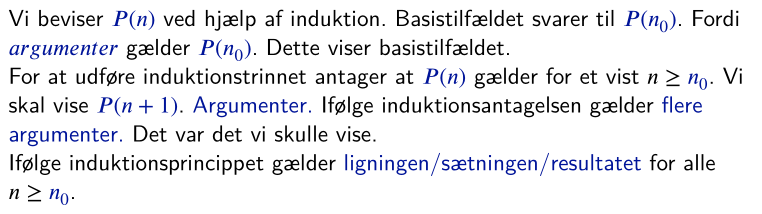
\includegraphics[width=1.0\textwidth]{Opg3/fig/3a_skabelon.png}
%\caption{Visualisering af legale ord. Rækkefølgen %af bogstaver er $(n-2) \quad (n-1) \quad n$.}
%\label{fig:2a}
%\end{figure}

Vi betragter for $n \in \mathbb{N}$ funktionen $f(n)$ defineret ved 

\begin{equation}
\label{eq:def}
f(n) = \sum_{k=0}^{n} 2^k
\end{equation}

Vi vil bevise ved induktion at der for alle $n \in \mathbb{N}$ gælder 

\begin{equation}
    f(n) = 2^{n+1} -1
\end{equation}

\textbf{Basistilfælde}\\
Basistilfældet svarer for $n_0 = 0$ til
\begin{equation}
    f(0)= 2^{0+1} -1=2-1 = 1
\end{equation}


Vi indsætter $n=0$ i definitionen \ref{eq:def}:
\begin{equation}
f(0) = \sum_{k=0}^{0} 2^k = 2^0 = 1
\end{equation}

Definitionen og induktionsantagelsen giver samme resultat. Dette viser basistilfældet.\\
\\
\textbf{Induktionstrin}\\
For at udføre induktionstrinnet antager vi at $f(n) = 2^{n+1} -1$ gælder for et $n \geq n_0$. Vi skal vise at $f(n+1)=2^{(n+1)+1} -1 = 2^{n+2} -1$. Dvs. hvis formlen virker for $n$, skal den også virke for $n+1$.\\
\\
Vi beregner $f(n+1)$ via definitionen, og tager det sidste led ud af summen:
\begin{equation}
f(n+1)= \sum_{k=0}^{n+1} 2^k = 2^{n+1} + \textcolor{red}{\sum_{k=0}^{n} 2^k}
\end{equation}

Vi anvender induktionsantagelsen, og substituerer:

\begin{equation}
f(n+1) = 2^{n+1} + \textcolor{red}{2^{n+1}-1}
\end{equation}

Vi simplificerer ved brug af eksponentregler:

\begin{equation}
f(n+1) = 2 \cdot 2^{n+1} -1 = 2^{n+2} -1
\end{equation}

Dvs. ifølge induktionsagelsen gælder $f(n+1) = 2^{n+2} -1$. Det var det, vi skulle vise. \\
\\
\textbf{Konklusion}\\
Ifølge induktionsprincippet gælder da $f(n) = 2^{n+1} -1$ for alle $n \geq n_0$. Da $n_0 = 0$, gælder formlen således for alle $n \in \mathbb{N}$. 
